











%----REGULARIZACE------------------------------------------------------------------------------------
\section{Regularizace}
\label{sec:Regularizace}
















%----PROBLEM-PRETRENOVANI---------------------------------------------------------------------------
\subsection{Problém přetrénování}
\label{sec:RegularizaceProblemPretrenovani}

\par{Nyní když známe algoritmy lineární a binární regrese, které se hodí pro řešení mnoha úloh strojového učení, musíme si říci něco o problému zvaném přetrénování. Tento problém způsobuje, že dané algoritmy ve výsledku fungují velmi špatně.}

\par{V této sekci si vysvětlíme v čem problém přetrénování spočívá a v následujících sekcích bude popsán postup jak se s daným problémem vypořádat.}

\par{Vraťme se k našemu problému predikce ceny velikosti bytu, ve kterém jsme využili algoritmu lineární regrese.}

\par{Na Obr.~\ref{fig:regrese_0} jsou znázorněná trénovací data. Pokud využijeme lineární regresi společně s hypotézou $h_{\bm{\Theta}} \left( \bm{x} \right) = \vartheta_0 + \vartheta_1 x$, tak získáme predikci ve tvaru, který lze vidět na Obr. \ref{fig:regrese_1}. V tomto případě naše zvolená hypotéza $h_{\bm{\Theta}} \left( \bm{x} \right)$ nerespektuje dostatečně tvar našich trénovacích dat. Přesnější anglický termín pro takto nastalou situaci zní \textit{underfit} nebo \textit{high bias}, což se dá vysvětlit jako problém, kdy se snažíme použít regresi na trénovací data s~málo komplexní hypotézou. Tedy hypotéza nemůže dostatečně přesně vystihovat tvar dat (nezobecňuje).}
\begin{figure}[!ht]
	\centering
	\begin{minipage}[t]{0.48\textwidth}
  		%trim option's parameter order: left bottom right top
		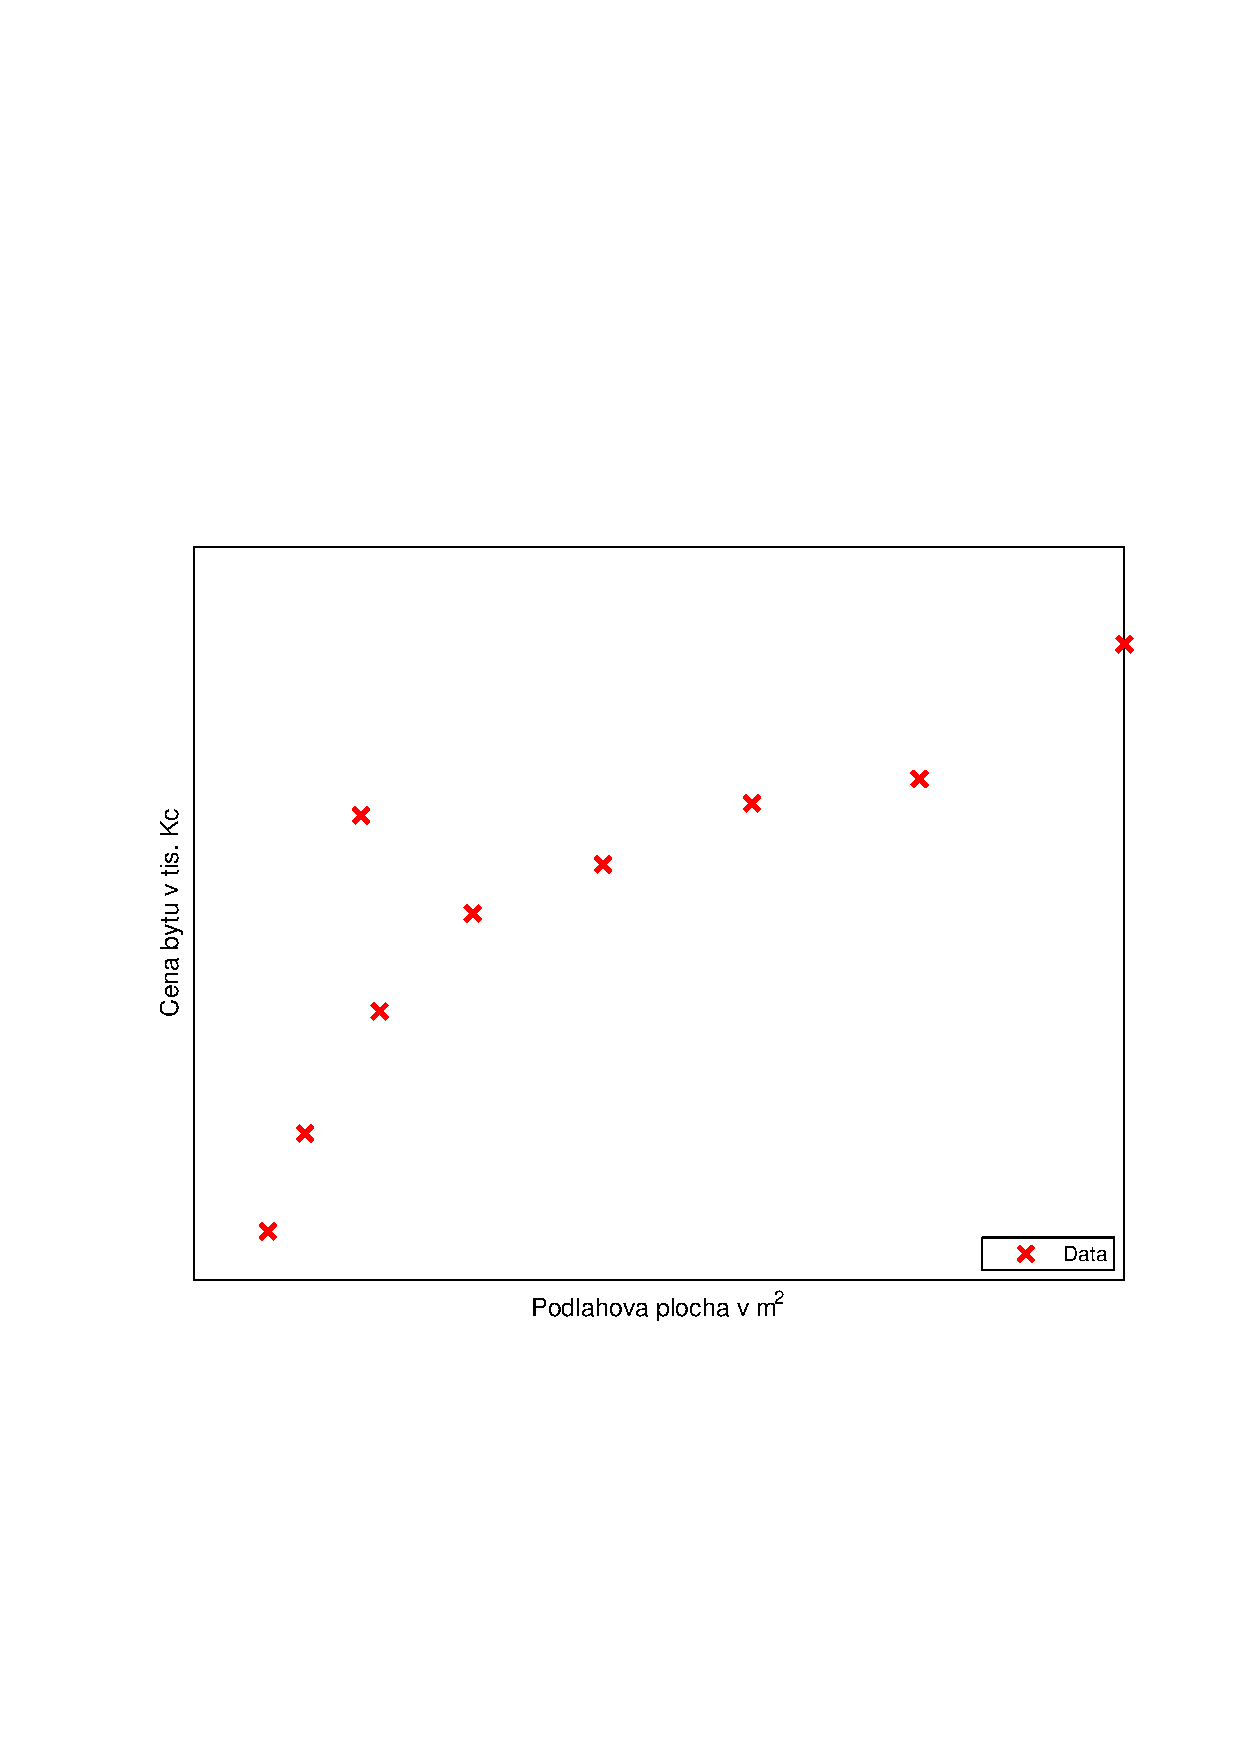
\includegraphics[width = \textwidth, trim = 2.5cm 7cm 2cm 9cm]{./Img/Regularizace/Pretrenovani1D/regrese_0.pdf}
  		\caption{Trénovací data.}
		\label{fig:regrese_0}
	\end{minipage}%
	\hfill
	\begin{minipage}[t]{0.48\textwidth}
		%trim option's parameter order: left bottom right top
		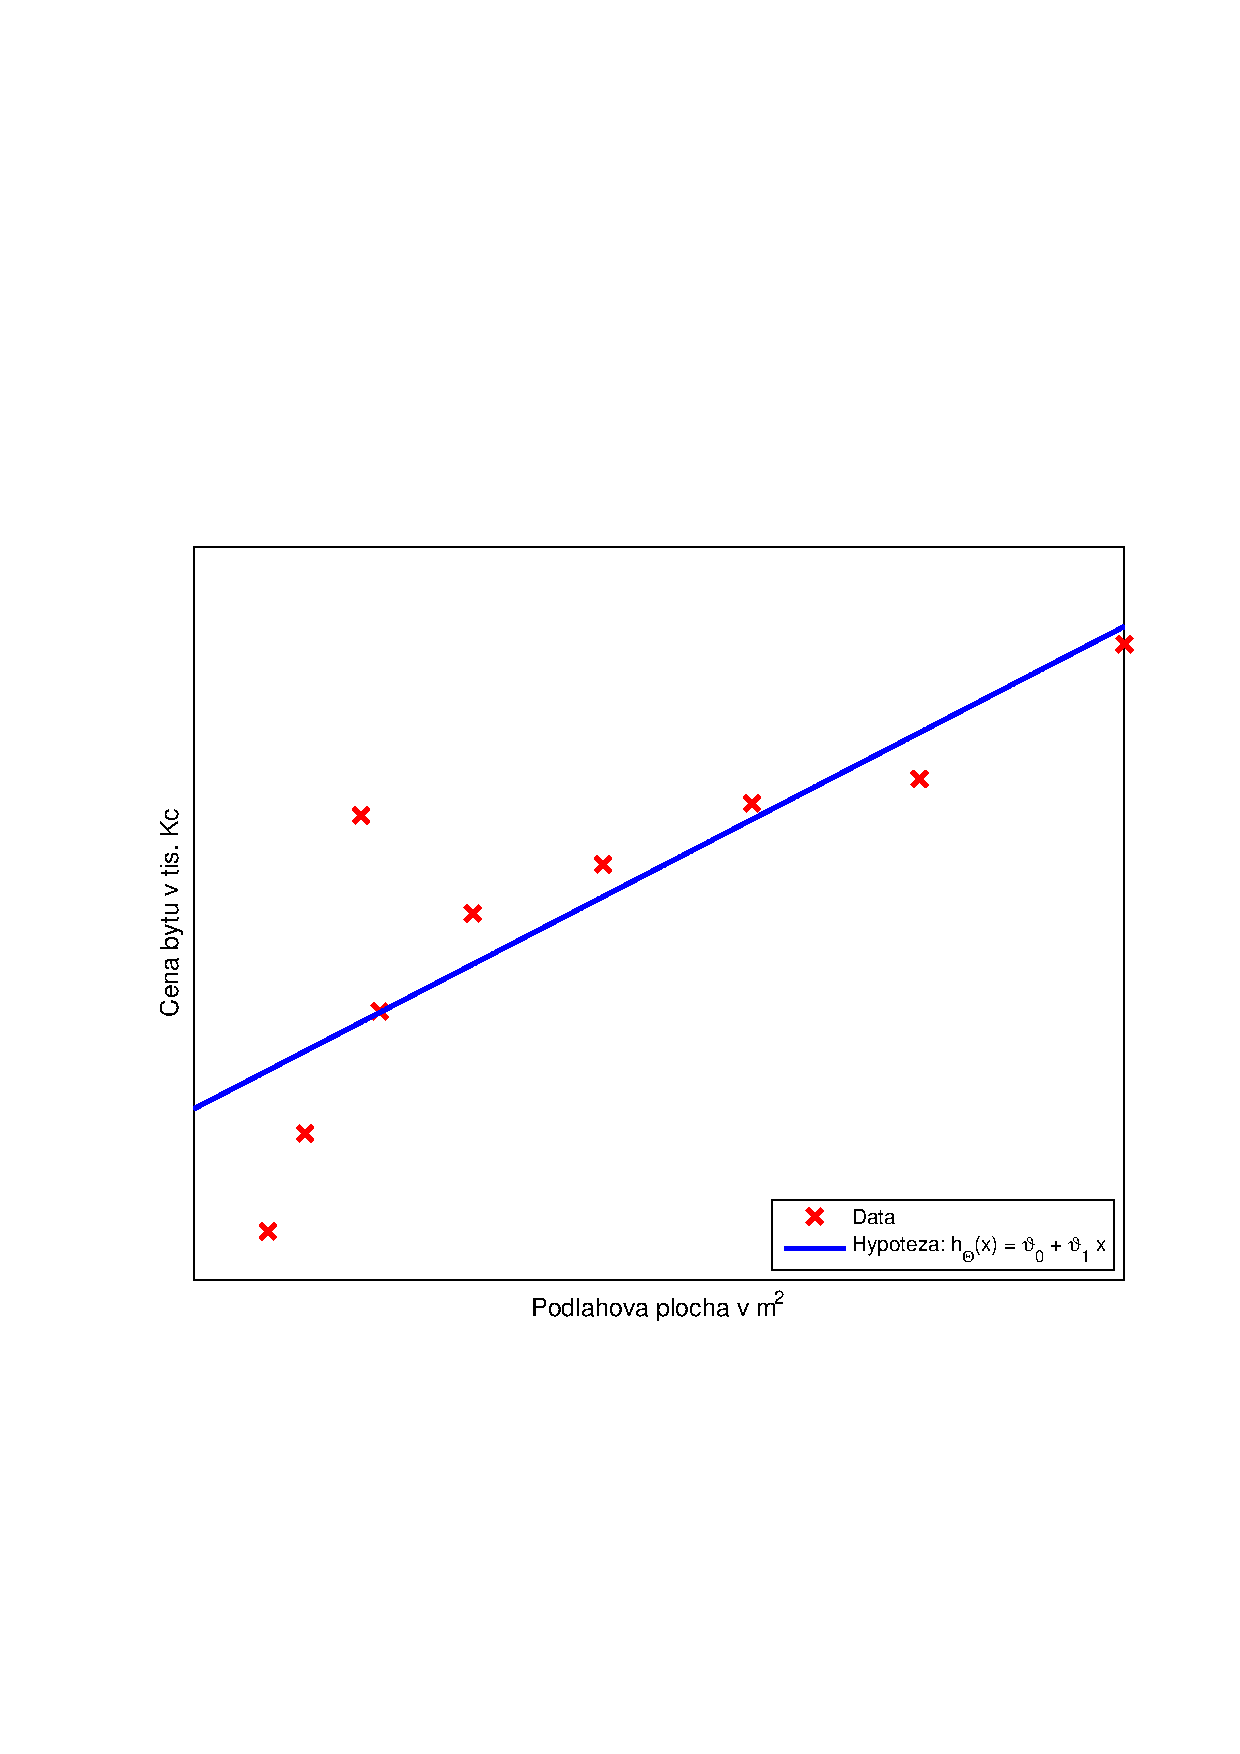
\includegraphics[width = \textwidth, trim = 2.5cm 7cm 2cm 9cm]{./Img/Regularizace/Pretrenovani1D/regrese_1.pdf}
  		\caption{Lineární regrese (\textit{underfit}, \textit{high bias}).}	
		\label{fig:regrese_1}
	\end{minipage}%
\end{figure}
\pagebreak

\par{Na Obr. \ref{fig:regrese_2} lze vidět regresi s hypotézou ve tvaru $h_{\bm{\Theta}} \left( \bm{x} \right) = \vartheta_0 + \vartheta_1 x + \vartheta_2 x^2$, která velmi dobře zobecňuje trénovací data a proto by byla v tomto případě nejlepší volbou.}

\par{Dále na Obr. \ref{fig:regrese_4} lze vidět regresi s hypotézou $h_{\bm{\Theta}} \left( \bm{x} \right) = \vartheta_0 + \vartheta_1 x + \vartheta_2 x^2 + \vartheta_2 x^3 + \vartheta_2 x^4$, jejíž chování je velmi \uv{divoké} a nezobecňuje trénovací data. V tomto případě se snaží hypotéza co nejvíce respektovat trénovací data za cenu ztráty obecnosti. Tento problém se nazývá přetrénování, anglicky \textit{overfitting} nebo \textit{high variance}.}

\begin{figure}[!ht]
	\centering
	\begin{minipage}[t]{0.48\textwidth}
  		%trim option's parameter order: left bottom right top
		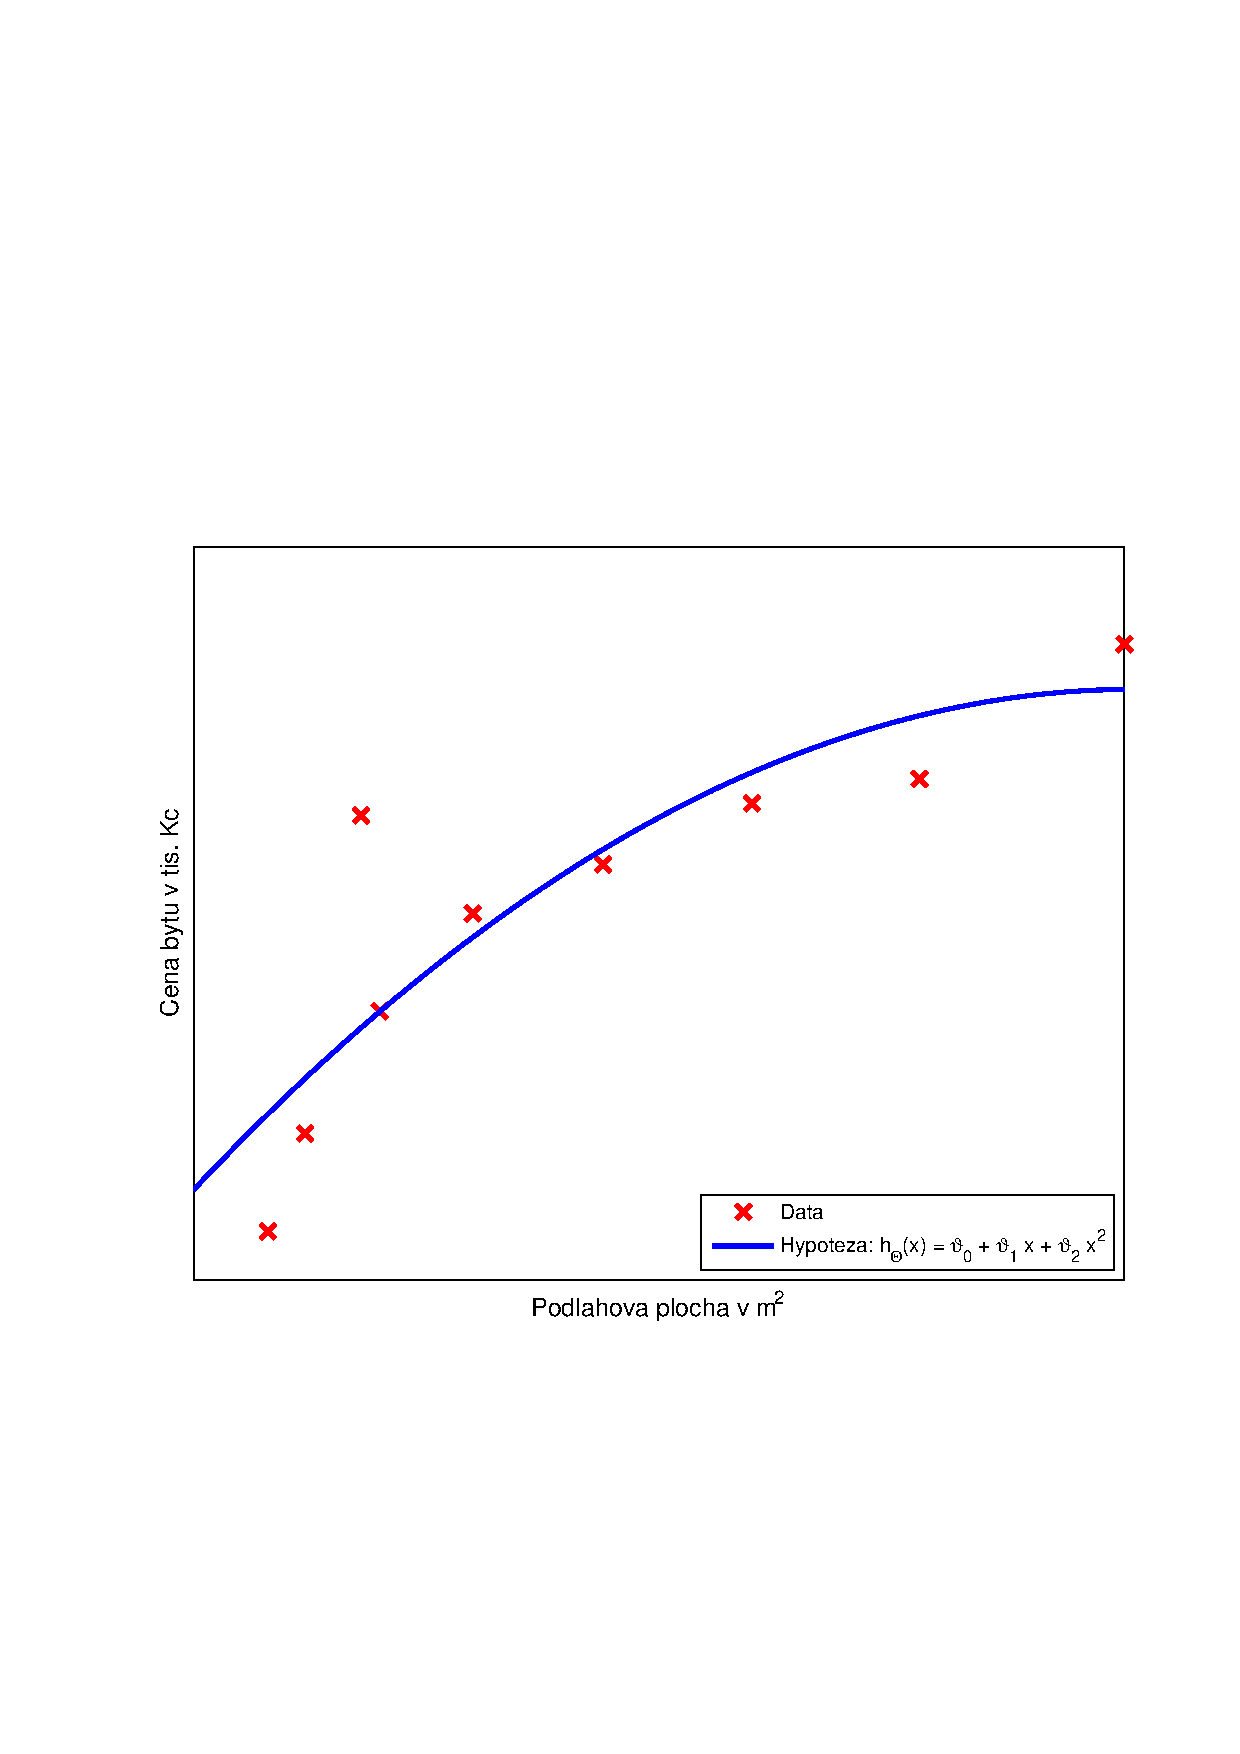
\includegraphics[width = \textwidth, trim = 2.5cm 7cm 2cm 9cm]{./Img/Regularizace/Pretrenovani1D/regrese_2.pdf}
  		\caption{Regrese pomocí hypotézy ve tvaru polynomu druhého stupně (\textit{just right}).}
		\label{fig:regrese_2}
	\end{minipage}%
	\hfill
	\begin{minipage}[t]{0.48\textwidth}
		%trim option's parameter order: left bottom right top
		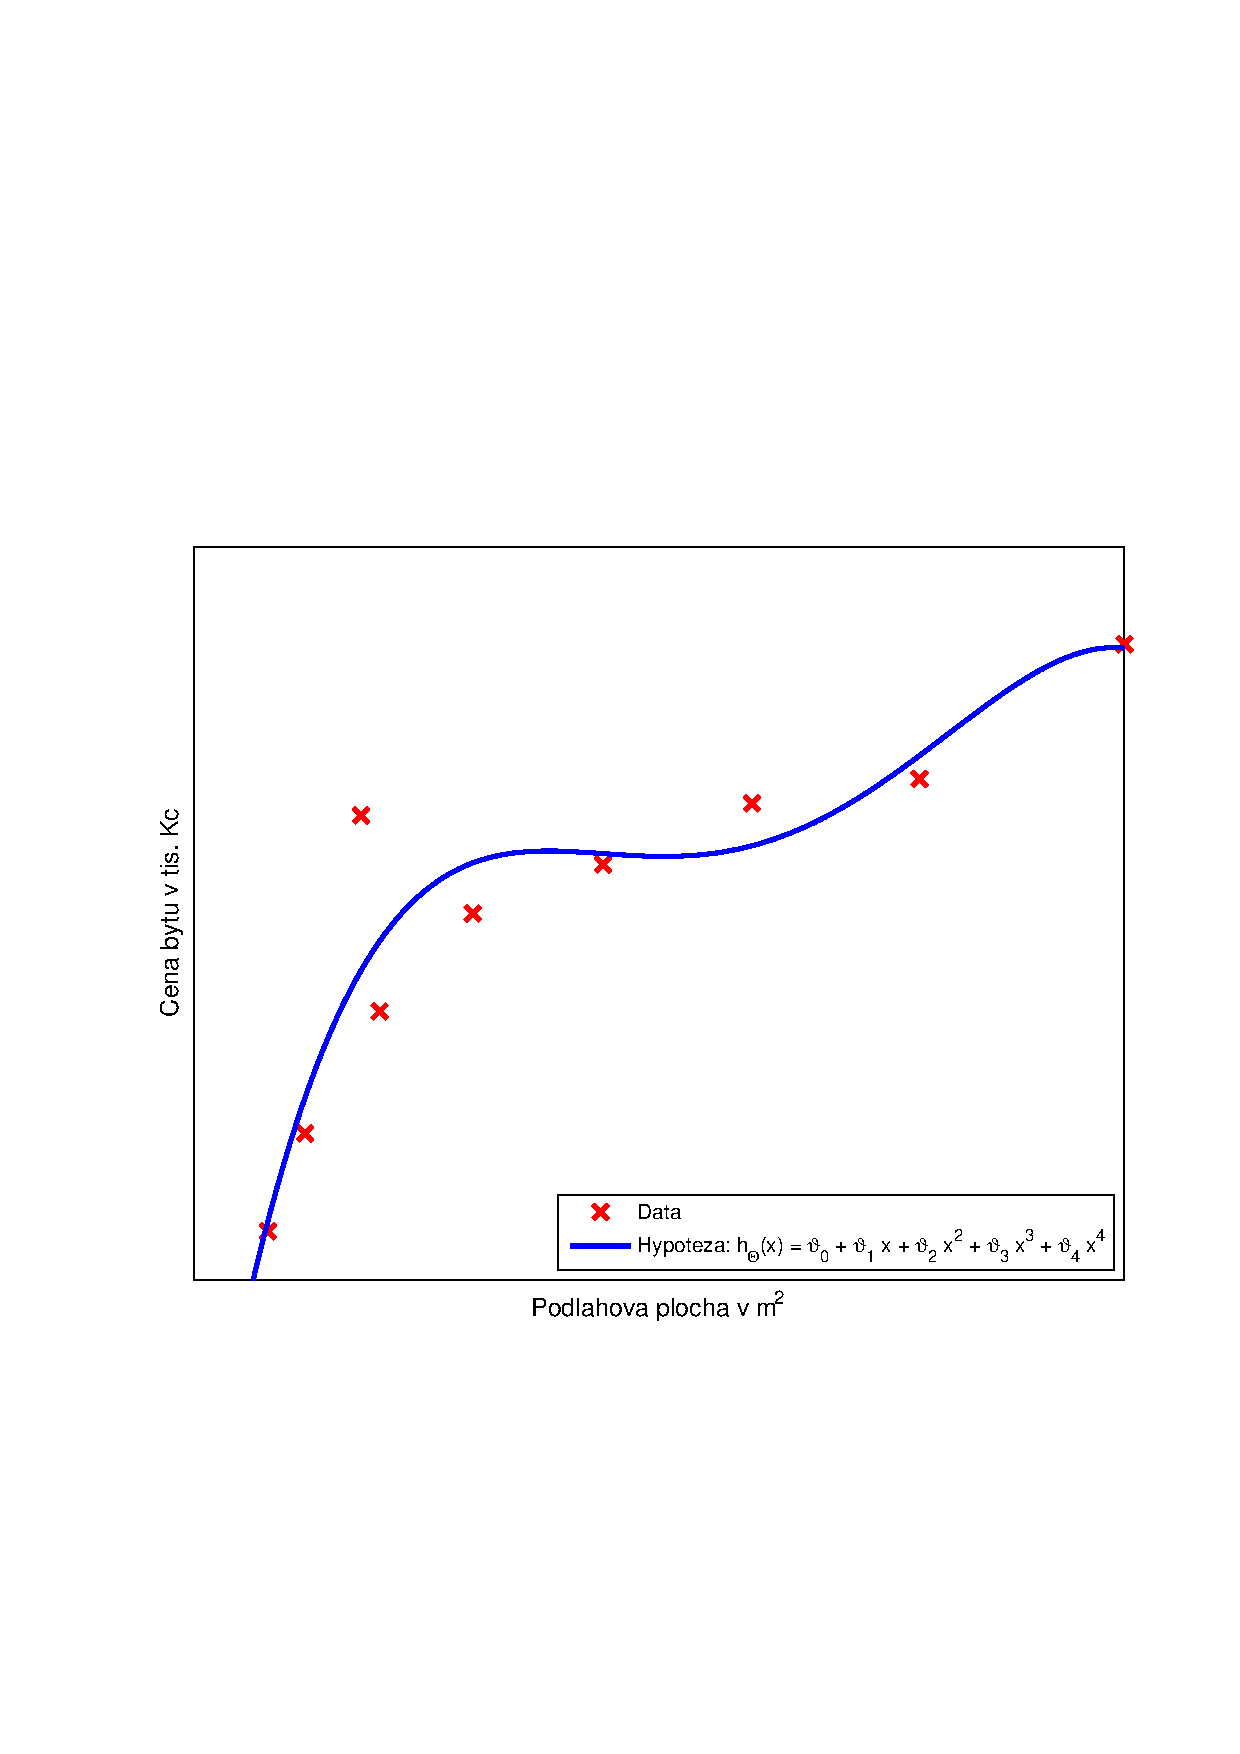
\includegraphics[width = \textwidth, trim = 2.5cm 7cm 2cm 9cm]{./Img/Regularizace/Pretrenovani1D/regrese_4.pdf}
  		\caption{Regrese pomocí hypotézy ve tvaru polynomu čtvrtého stupně (\textit{overfitting}, \textit{high variance}).}
		\label{fig:regrese_4}
	\end{minipage}%
\end{figure}

\subsubsection*{Přetrénování (\textit{overfitting}):}
\par{V případě, že máme příliš mnoho příznaků, hypotéza může velmi dobře respektovat trénovací data $\left( J \left( \bm{\Theta} \right) = \frac{1}{2m} \sum_{i=1}^{m} \left( h_{\bm{\Theta}} \left( \bm{x}^{\left( i \right)} \right) - y^{\left( i \right)} \right)^2 \approx 0 \right)$, ale nebude schopna správně klasifikovat nově příchozí vzorky. Nebude schopna generalizovat, tedy predikce na nově příchozích vzorcích selže.}

\subsubsection*{Možnosti odstranění přetrénování:}
\begin{enumerate}
	\item Redukovat počet příznaků.
		\begin{itemize}
			\item Manuálně zvolit příznaky, které budou zachovány.
			\item Automatická redukce příznaků například PCA.
		\end{itemize}
	\item Regularizace.
		\begin{itemize}
			\item Zachovat všechny příznaky, ale redukovat velikost / váhu parametrů $\vartheta_j$.
			\item Funguje správně pokud máme velké množství příznaků, kde každý malou měrou přispívá k predikci $y$.
		\end{itemize}				
\end{enumerate}



\newpage

















%----ZTRATOVA-FUNKCE-------------------------------------------------------------------------
\subsection{Ztrátová funkce}
\par{V sekci \ref{sec:RegularizaceProblemPretrenovani} jsme si ukázali jak lze pomocí kvadratické hypotézy $h_{\bm{\Theta}} \left( \bm{x} \right) = \vartheta_0 + \vartheta_1 x + \vartheta_2 x^2$ dobře zobecnit naše trénovací data. Dále již víme, že hypotéza ve tvaru $h_{\bm{\Theta}} \left( \bm{x} \right) = \vartheta_0 + \vartheta_1 x + \vartheta_2 x^2 + \vartheta_2 x^3 + \vartheta_2 x^4$ nezobecňuje naší trénovací množinu dat dobře.}
\begin{figure}[!ht]
	\centering
	\begin{minipage}[t]{0.48\textwidth}
  		%trim option's parameter order: left bottom right top
		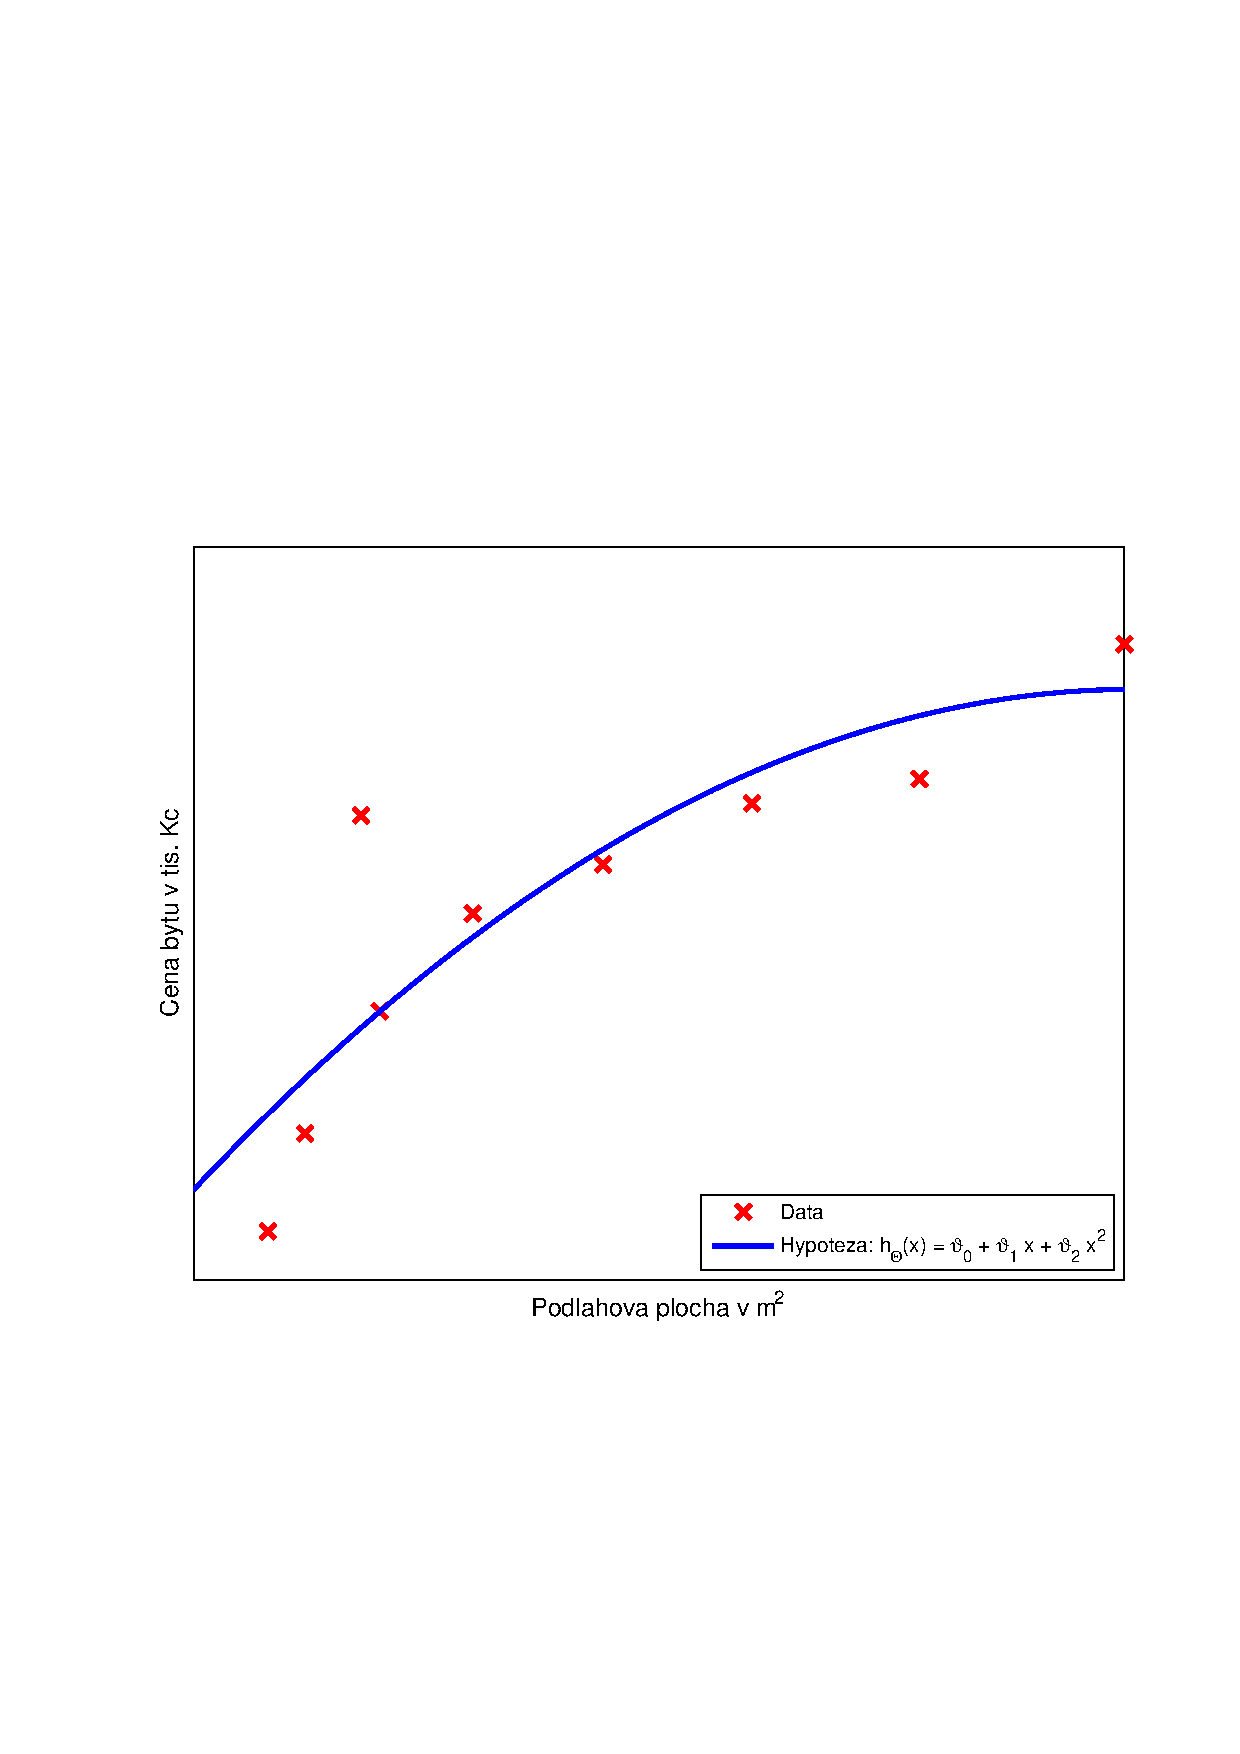
\includegraphics[width = \textwidth, trim = 2.5cm 7cm 2cm 9cm]{./Img/Regularizace/Pretrenovani1D/regrese_2.pdf}
  		\caption{Regrese pomocí hypotézy ve tvaru polynomu druhého stupně (\textit{just right}).}
	\end{minipage}%
	\hfill
	\begin{minipage}[t]{0.48\textwidth}
		%trim option's parameter order: left bottom right top
		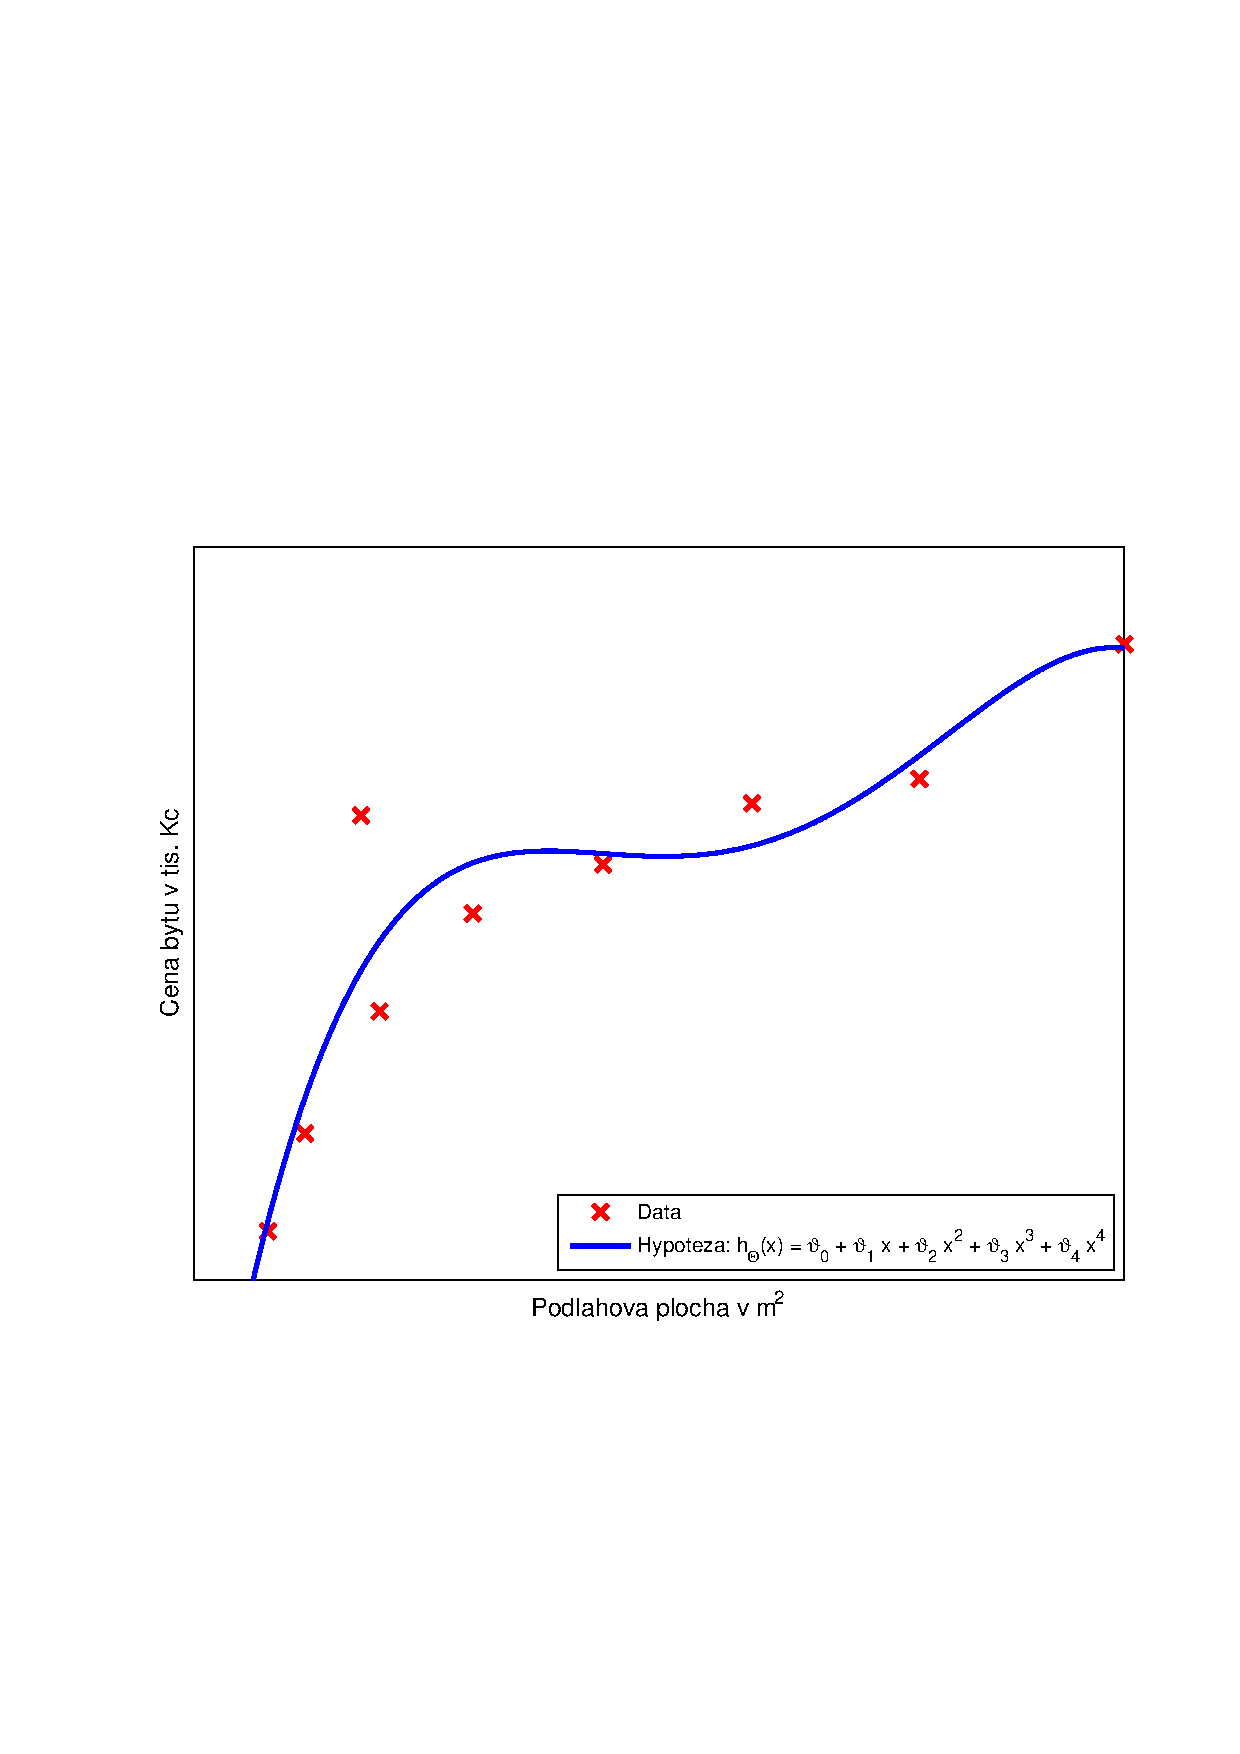
\includegraphics[width = \textwidth, trim = 2.5cm 7cm 2cm 9cm]{./Img/Regularizace/Pretrenovani1D/regrese_4.pdf}
  		\caption{Regrese pomocí hypotézy ve tvaru polynomu čtvrtého stupně (\textit{overfitting}, \textit{high variance}).}
	\end{minipage}%
\end{figure}

\par{Předpokládejme, že budeme penalizovat parametry $\vartheta_3$ a $\vartheta_4$ (jejich hodnoty budou malé). V rovnici \ref{eq:minZtratovaFunkce} je ukázána naše známá optimalizace
\begin{equation}
	\min_{\bm{\Theta}} \frac{1}{2m} \sum_{i=1}^{m} \left( h_{\bm{\Theta}} \left( \bm{x}^{\left( i \right)} \right) - y^{\left( i \right)} \right)^2,
	\label{eq:minZtratovaFunkce}
\end{equation}
kterou můžeme upravit na tvar
\begin{equation}
	\min_{\bm{\Theta}} \frac{1}{2m} \sum_{i=1}^{m} \left( h_{\bm{\Theta}} \left( \bm{x}^{\left( i \right)} \right) - y^{\left( i \right)} \right)^2 + 1000 \vartheta_3^2 + 1000 \vartheta_4^2,
	\label{eq:minZtratovaFunkce1000}
\end{equation}
kde hodnoty 1000 jsou pouze ilustrativní a~reprezentují velká čísla (velké váhy). Tedy pokud bychom chtěli minimalizovat rovnici \ref{eq:minZtratovaFunkce1000}, tak to lze za předpokladu, že $\vartheta_3$ a~$\vartheta_4$ budou malá čísla. V případě, že $\vartheta_3 \approx 0$ a $\vartheta_4 \approx 0$, tak získáme opět náš minimalizační problém jako v~rovnici \ref{eq:minZtratovaFunkce}. Ještě větší dopad to má na tvar hypotézy $h_{\bm{\Theta}} \left( \bm{x} \right) = \vartheta_0 + \vartheta_1 x + \vartheta_2 x^2 + \vartheta_2 x^3 + \vartheta_2 x^4$, která dříve vedla k přetrénování. Ta v~případě, že  $\vartheta_3 \approx 0$ a $\vartheta_4 \approx 0$ přejde na tvar $h_{\bm{\Theta}} \left( \bm{x} \right) = \vartheta_0 + \vartheta_1 x + \vartheta_2 x^2$. Tímto se zbavíme problému přetrénování a~získáme tvar hypotézy, který dobře zobecňuje trénovací data.}

\subsubsection*{Regularizace}
\par{Čím jsou menší hodnoty parametrů $\vartheta_0,\vartheta_1, \ldots , \vartheta_n$, tím \uv{jednodušší} tvar hypotézy získáme a tím méně je tvar hypotézy náchylný k přetrénování. Zapsáno rovnicí
\begin{equation}
	J \left( \bm{\Theta} \right) = \frac{1}{2m} \left( \sum_{i = 1}^{m} \left( h_{\bm{\Theta}} \left( \bm{x}^{\left( i \right)} \right) - y^{\left( i \right)} \right)^2 + \lambda \sum_{j = 1}^{n} \vartheta_j^2 \right),
\end{equation}
kde je nejdříve podotknout, že nová suma s indexem $j$ má jinou mez $n$ než první suma. To je způsobeno tím, že se regularizace vztahuje pouze na parametry $\vartheta_1, \vartheta_2, \ldots , \vartheta_m$, tedy parametr $\vartheta_0$ není regularizován, protože je vždy násoben jedničkou, nepřijde do kontaktu s~příznaky vzorků. Dále parametr $\lambda$ je takzvaný regularizační parametr, který kontroluje vyvážení mezi tím, jak hodně bude regularizace ovlivňovat původní ztrátovou funkci $J \left( \bm{\Theta} \right)$. Regularizace je dána vztahem 
\begin{equation}
	\lambda \sum_{j = 1}^{n} \vartheta_j^2.
\end{equation}
Našim cílem je jako dříve minimalizovat ztrátovou funkci
\begin{equation}
	\min_{\bm{\Theta}} J \left( \bm{\Theta} \right)
\end{equation}}

\par{Co se stane, pokud bude regularizační parametr $\lambda$ příliš velký? Řekněme, že $\lambda = 10^{10}$. Poté hypotéza ve tvaru $h_{\bm{\Theta}} \left( \bm{x} \right) = \vartheta_0 + \vartheta_1 x + \vartheta_2 x^2 + \vartheta_2 x^3 + \vartheta_2 x^4$ přejde na tvar $h_{\bm{\Theta}} \left( \bm{x} \right) = \vartheta_0$ a~výsledný průběh lze vidět na Obr.~\ref{fig:regularizaceUnderfit}}
\begin{figure}[!ht]
	\centering
	%trim option's parameter order: left bottom right top
	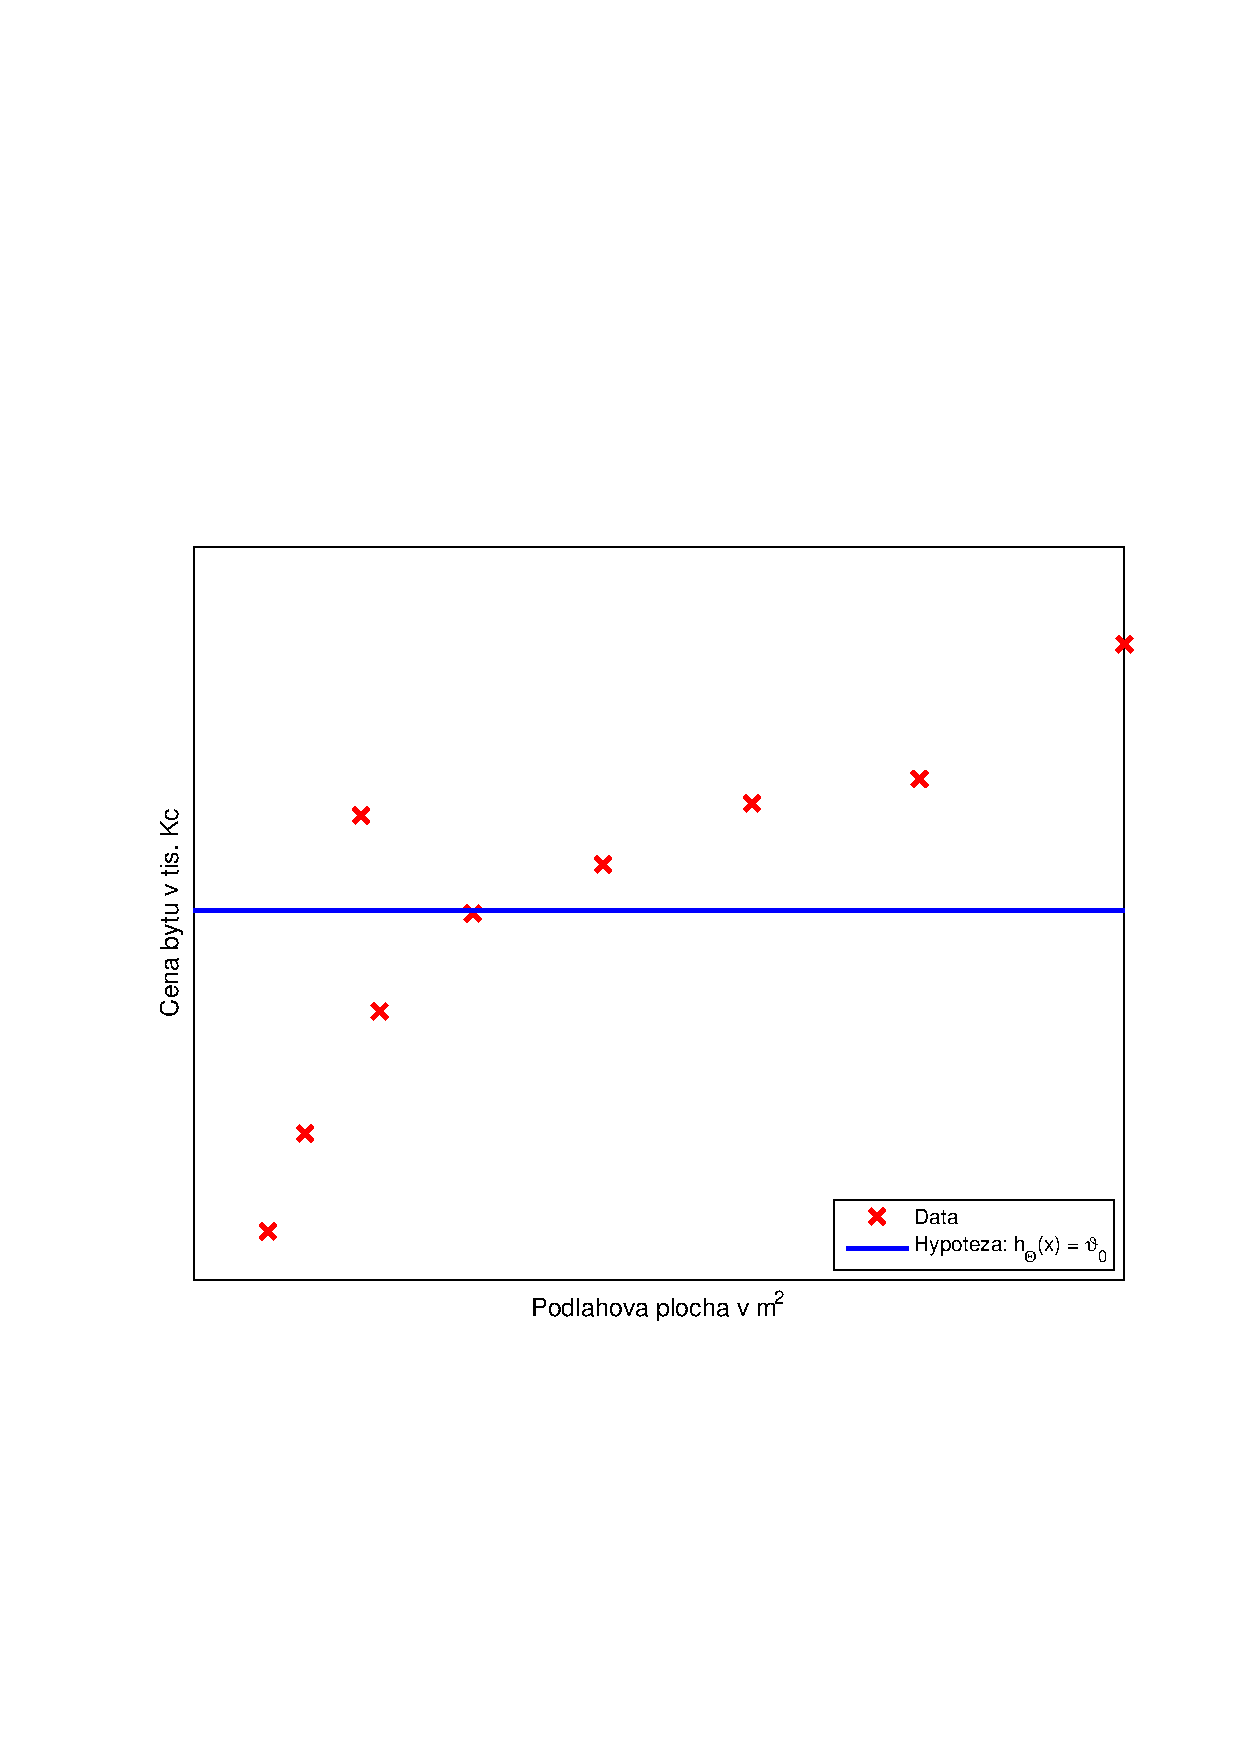
\includegraphics[width = 0.48\textwidth, trim = 2.5cm 7cm 2cm 9cm]{./Img/Regularizace/ZtratovaFunkce/regrese_underfit.pdf}
	\caption{Použití regularizace k získání \textit{underfit} hypotézy.}
	\label{fig:regularizaceUnderfit}
\end{figure}

\par{Z~uvedeného vyplývá, že je nutné volit regularizační parametr~$\lambda$ velmi opatrně. S~velkým~$\lambda$ dosáhneme \textit{underfit} problému a~s~malým~$\lambda$ neodstraníme \textit{overfit} problém.}

\newpage

















%----REGULARIZACE-LINEARNI-REGRESE--------------------------------------------------------------
\subsection{Regularizace lineární regrese}
\label{sec:RegularizaceLinearniRegrese}

\par{Pro lineární regresi máme odvozen gradientní algoritmus a analytické řešení. V této sekci oba algoritmy zobecníme s využitím regularizace.}


\subsubsection*{Regularizace gradientního algoritmu lineární regrese}
\par{Máme naší optimalizační úlohu lineární regrese společně s regularizací
\begin{equation}
	J \left( \bm{\Theta} \right) = \frac{1}{2m} \left( \sum_{i = 1}^{m} \left( h_{\bm{\Theta}} \left( \bm{x}^{\left( i \right)} \right) - y^{\left( i \right)} \right)^2 + \lambda \sum_{j = 1}^{n} \vartheta_j^2 \right),
\end{equation}
snažíme se minimalizovat ztrátovou funkci 
\begin{equation}
	\min_{\bm{\Theta}} J \left( \bm{\Theta} \right)
\end{equation}}

\par{Připomeňme si dříve představený gradientní algoritmus lineární regrese. Opakuj
\begin{equation}
	\vartheta_j = \vartheta_j - \alpha \frac{1}{m} \sum_{i = 1}^{m} \left( h_{\bm{\Theta}} \left( \bm{x}^{\left( i \right)} \right) - y^{\left( i \right)} \right) x_j^{\left( i \right)}, \quad j = 0,1,\ldots ,n .
\end{equation}
Tento algoritmus je možno rozdělit do dvou kroků. Rozdělit výpočet pro $\vartheta_0$ a $\vartheta_{1,\ldots, n}$. Opakuj
\begin{eqnarray}
	&\vartheta_0 &= \vartheta_0 - \alpha \frac{1}{m} \sum_{i = 1}^{m} \left( h_{\bm{\Theta}} \left( \bm{x}^{\left( i \right)} \right) - y^{\left( i \right)} \right) x_0^{\left( i \right)},\\
	%
	&\vartheta_j &= \vartheta_j - \alpha \frac{1}{m} \sum_{i = 1}^{m} \left( h_{\bm{\Theta}} \left( \bm{x}^{\left( i \right)} \right) - y^{\left( i \right)} \right) x_j^{\left( i \right)}, \quad j = 1,2,\ldots ,n .
\end{eqnarray}
Doposud na algoritmu nebylo nic změněno, pouze byl rozepsán do dvou kroků. Protože víme, že na parametr $\vartheta_0$ se regularizace nevztahuje, proto můžeme algoritmus pozměnit a přidat regularizační člen. Následně bude mít gradientní algoritmus tvar. Opakuj
\begin{eqnarray}
	&\vartheta_0 &= \vartheta_0 - \alpha \frac{1}{m} \sum_{i = 1}^{m} \left( h_{\bm{\Theta}} \left( \bm{x}^{\left( i \right)} \right) - y^{\left( i \right)} \right) x_0^{\left( i \right)},\\
		%
	&\vartheta_j &= \vartheta_j - \alpha \left( \frac{1}{m} \sum_{i = 1}^{m} \left( h_{\bm{\Theta}} \left( \bm{x}^{\left( i \right)} \right) - y^{\left( i \right)} \right) x_j^{\left( i \right)} + \frac{\lambda}{m} \vartheta_j \right), \quad j = 1,2,\ldots ,n,	
	\label{eq:LinearniRegreseGradientniAlgProJ1}
\end{eqnarray}
kde platí
\begin{eqnarray}
	\frac{\partial}{\partial \vartheta_0} &J \left( \bm{\Theta} \right)	&= \left( \frac{1}{m} \sum_{i = 1}^{m} \left( h_{\bm{\Theta}} \left( \bm{x}^{\left( i \right)} \right) - y^{\left( i \right)} \right) x_0^{\left( i \right)} \right),\\
	%
	\frac{\partial}{\partial \vartheta_j} &J \left( \bm{\Theta} \right) &= \left( \frac{1}{m} \sum_{i = 1}^{m} \left( h_{\bm{\Theta}} \left( \bm{x}^{\left( i \right)} \right) - y^{\left( i \right)} \right) x_j^{\left( i \right)} + \frac{\lambda}{m} \vartheta_j \right), \quad j = 1,2,\ldots ,n.
\end{eqnarray}}

\par{Rovnice \ref{eq:LinearniRegreseGradientniAlgProJ1} lze přepsat do tvaru 
\begin{equation}
	\vartheta_j = \vartheta_j \left( 1 - \alpha \frac{\lambda}{m} \right) - \alpha \frac{1}{m} \sum_{i = 1}^{m} \left( h_{\bm{\Theta}} \left( \bm{x}^{\left( i \right)} \right) - y^{\left( i \right)} \right) x_j^{\left( i \right)},
\end{equation}
kde platí
\begin{equation}
	1 - \alpha \frac{\lambda}{m} < 1.
\end{equation}}



\subsubsection*{Regularizace analytického řešení lineární regrese}

\par{Připomeňme si}
\begin{equation}
	\bm{X} = \left[ \left( \bm{x}^{\left( 1 \right)} \right)^{\top}, \ldots, \left( \bm{x}^{\left( m \right)} \right)^{\top}  \right]^{\top},\quad  \bm{X} \in  \mathcal{R}^{m \times \left( n + 1 \right)}
\end{equation}
a
\begin{equation}
	\bm{y} = \left[ y^{\left( 1 \right)}, \ldots, y^{\left( m \right)}   \right]^{\top}, \quad \bm{y} \in \mathcal{R}^{m}.
\end{equation}
Analytické řešení pro výpočet $\bm{\Theta}$ má tvar
\begin{equation}
	\bm{\Theta} = \left( \bm{X}^{\top} \bm{X} \right)^{-1} \bm{X}^{\top} y.
\end{equation}
Cílem je minimalizovat ztrátovou funkci
\begin{equation}
	\min_{\bm{\Theta}} J \left( \bm{\Theta} \right).
\end{equation}

\par{Pokud využijeme regularizaci, tak naše analytické řešení přejde na tvar
\begin{equation}
	\bm{\Theta} = \left( \bm{X}^{\top} \bm{X} + \lambda 
	\left[ \begin{array}{ccccc}
		0 & 0 & 0 & 0 & 0\\
		0 & 1 & 0 & 0 & 0 \\
		0 & 0 & 1 & 0 & 0\\
		0 & 0 & 0 & \ddots & \vdots\\
		0 & 0 & 0 & \cdots & 1
	\end{array} \right] \right)^{-1} \bm{X}^{\top} y
\end{equation}
kde nová matice má velikost $\mathcal{R}^{\left( n + 1 \right) \times \left( n+ 1 \right)}$}

\subsubsection*{Rozšíření}
\par{Předpokládejme, že $m \leq n$, kde $m$ je počet vzorků a $n$ je počet příznaků a 
\begin{equation}
	\bm{\Theta} = \left( \bm{X}^{\top} \bm{X} \right)^{-1} \bm{X}^{\top} y,
\end{equation}
pak je matice $\bm{X}^{\top} \bm{X} $ neinvertovatelná / singulární.}

\par{Pro výpočet lze v tomto případě využít pseudoinverze, konkrétně v~MATLABu k~tomuto účelu slouží funkce \textit{pinv()}.}
\lstinputlisting[language = Matlab]{./Img/Regularizace/noninvertibilityXX/XX.m}

\par{Pokud $\lambda > 0$}
\begin{equation}
	\bm{\Theta} = \left( \underbrace{ \bm{X}^{\top} \bm{X} + \lambda 
	\left[ \begin{array}{ccccc}
		0 & ~ & ~ & ~ & ~\\
		~ & 1 & ~ & ~ & ~ \\
		~ & ~ & 1 & ~ & ~\\
		~ & ~ & ~ & \ddots & ~\\
		~ & ~ & ~ & ~ & 1
	\end{array} \right]}_{\text{Matice musí být invertovatelná}}  \right)^{-1} \bm{X}^{\top} y
\end{equation}

\newpage






















%----REGULARIZACE-BINARNI REGRESE--------------------------------------------------------------
\subsection{Regularizace binární regrese}
\par{Pro binární regresi jsme dříve mluvili o dvou typech optimalizace. Mluvili jsme o tom, jak použít gradientní algoritmus a jak použít pokročilé metody optimalizace. V této sekci si ukážeme, jak tyto přístupy upravit, aby využily regularizace.}

\subsubsection*{Regularizace binární regrese}

\par{Dříve jsme si ukázali, že binární regrese je náchylná na přetrénování v případě, kdy zvolíme vysoký stupeň polynomu reprezentující naší hypotézu, například
\begin{equation}
	h_{\bm{\Theta}} \left( \bm{x} \right) = g \left( \vartheta_0  + \vartheta_1 x_1 + \vartheta_2 x^2_1 + \vartheta_3 x_1^2 x_2 + \vartheta_4 x_1^2 x_2^2 + \vartheta_5 x_1^2 x_2^3 + \ldots \right),
	\label{eq:BReg_hypo}
\end{equation}
pro takovouto složitou hypotézu můžeme dostat dělící křivku velmi variabilní a velmi respektující rozdělení trénovacích dat, tedy křivku, která nedostatečně zobecňuje.
\begin{figure}[!ht]
	\centering
	%trim option's parameter order: left bottom right top
	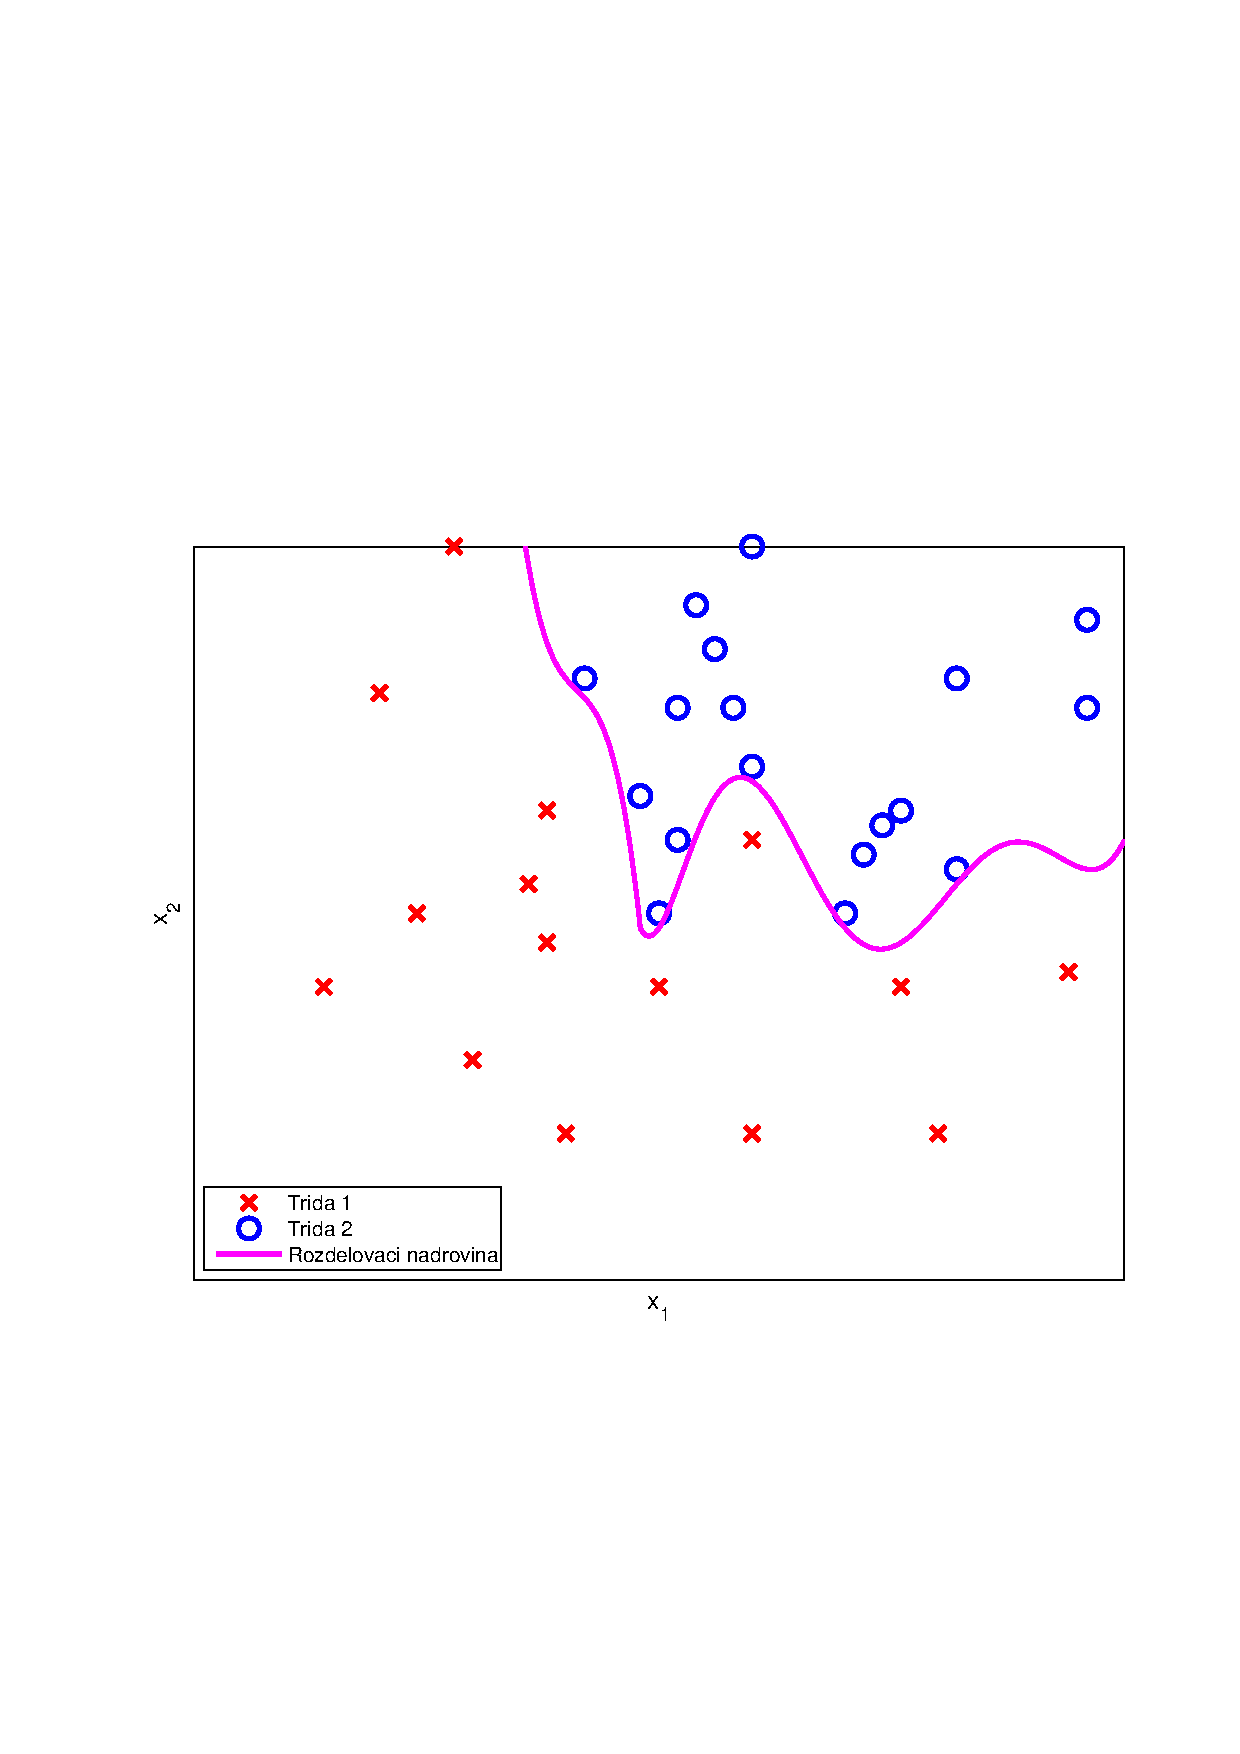
\includegraphics[width = 0.48\textwidth, trim = 2.5cm 7cm 2cm 9cm]{./Img/Regularizace/binarniRegrese/regularizace_binarni_regrese.pdf}
	\caption{Možný výsledek s použitím hypotézy z rovnice \ref{eq:BReg_hypo}.}
	\label{fig:binaryRegularizationExample}
\end{figure}
}

\par{Ztrátová funkce pro binární regresi má tvar
\begin{equation}
	J \left( \bm{\Theta} \right) =  - \left[ \frac{1}{m} \sum_{i = 1}^{m} y^{ \left( i \right)} \log \left( h_{\bm{\Theta}} \left( \bm{x}^{\left( i \right)} \right) \right) + \left( 1 - y^{\left( i \right)} \right) \log \left( 1 - h_{\bm{\Theta}} \left( \bm{x}^{\left( i \right)} \right) \right) \right]
\end{equation}
a její modifikací získáme regularizovaný tvar ztrátové funkce
\begin{equation}
	J \left( \bm{\Theta} \right) =  - \left[ \frac{1}{m} \sum_{i = 1}^{m} y^{ \left( i \right)} \log \left( h_{\bm{\Theta}} \left( \bm{x}^{\left( i \right)} \right) \right) + \left( 1 - y^{\left( i \right)} \right) \log \left( 1 - h_{\bm{\Theta}} \left( \bm{x}^{\left( i \right)} \right) \right) \right] + \frac{\lambda}{2m} \sum_{j = 1}^{n} \vartheta_j^2
\end{equation}
přidaná suma je jen do $n$, jelikož se neregularizuje složka $\vartheta_0$, která je vždy rovna jedné a~není v~součinu se žádnou proměnnou $x$, $y$. Tvar ztrátové funkce společně s~regularizací bude naší rozdělovací nadrovinu více zobecňovat a~pomůže nám řešit problém přetrénování.}

\par{Implementace bude provedena následovně: opakuj
\begin{eqnarray}
	&\vartheta_0 &= \vartheta_0 - \alpha \frac{1}{m} \sum_{i = 1}^{m} \left( h_{\bm{\Theta}} \left( \bm{x}^{\left( i \right)} \right) - y^{\left( i \right)} \right) x_0^{\left( i \right)}\\
	&\vartheta_j &= \vartheta_j - \alpha \left[ \frac{1}{m} \sum_{i = 1}^{m} \left( h_{\bm{\Theta}} \left( \bm{x}^{\left( i \right)} \right) - y^{\left( i \right)} \right) x_j^{\left( i \right)} + \frac{\lambda}{m} \vartheta_j \right], \qquad j = 1, 2, 3, \ldots , n,
	\label{eq:gradDescent_regularizace2rce}
\end{eqnarray}
kde 
\begin{equation}
	h_{\bm{\Theta}} \left( \bm{x} \right) = \frac{1}{1 + e^{- \bm{\Theta}^{\top} \bm{x} }}.
\end{equation}
Z~rovnice \ref{eq:gradDescent_regularizace2rce} lze vidět, že platí
\begin{equation}
	\frac{\partial}{\partial \vartheta_j} J \left( \bm{\Theta} \right) = \frac{1}{m} \sum_{i = 1}^{m} \left( h_{\bm{\Theta}} \left( \bm{x}^{\left( i \right)} \right) - y^{\left( i \right)} \right) x_j^{\left( i \right)} + \frac{\lambda}{m} \vartheta_j.
\end{equation}}





\subsubsection*{Regularizace pokročilé optimalizace}
\par{Nyní bude nastíněno jak využit pokročilé optimalizace v MATLABu. Nechť náš vektor parametrů $\bm{\Theta}$ odpovídá
\begin{equation}
	\bm{\Theta} = \left[ \vartheta_0 , \vartheta_1, \ldots , \vartheta_n \right]^{\top} = \left[ theta(1), theta(2), \ldots, theta(n + 1 ) \right]
\end{equation}
(z důvodu, že MATLAB indexuje od jedničky).
\lstinputlisting[language = Matlab]{./Img/Regularizace/AdvancedOptimalization/costFunction.m}
\begin{equation}
	J \left( \bm{\Theta} \right) = \left[ 
	- \frac{1}{m} \sum_{i = 1}^{m} y^{\left( i \right)} 
	\log \left( h_{\bm{\Theta}} \left( \bm{x}^{\left( i \right) } \right) \right)
	+ \left( 1 - y^{\left( i \right)} \right)
	\log \left( 1 - h_{\bm{\Theta}} \left( \bm{x}^{\left( i \right)} \right) \right) \right] + \frac{\lambda}{2m} \sum_{j = 1}^{n} \vartheta_j^2
\end{equation}
dále výpočet gradientu
\lstinputlisting[language = Matlab]{./Img/Regularizace/AdvancedOptimalization/grad1.m}
\begin{equation}
	\frac{\partial}{\partial \vartheta_0} J \left( \bm{\Theta} \right) = \frac{1}{m} \sum_{i = 1}^{m} \left( h_{\bm{\Theta}} \left( \bm{x}^{\left( i \right)} \right) - y^{\left( i \right)} \right) x_0^{\left( i \right)},
\end{equation}
\lstinputlisting[language = Matlab]{./Img/Regularizace/AdvancedOptimalization/grad2.m}
\begin{equation}
	\frac{\partial}{\partial \vartheta_1} J \left( \bm{\Theta} \right) = \left[ \frac{1}{m} \sum_{i = 1}^{m} \left( h_{\bm{\Theta}} \left( \bm{x}^{\left( i \right)} \right) - y^{\left( i \right)} \right) x_1^{\left( i \right)} \right] + \frac{\lambda}{m} \vartheta_1,
\end{equation}
\lstinputlisting[language = Matlab]{./Img/Regularizace/AdvancedOptimalization/grad3.m}
\begin{equation}
	\frac{\partial}{\partial \vartheta_2} J \left( \bm{\Theta} \right) = \left[ \frac{1}{m} \sum_{i = 1}^{m} \left( h_{\bm{\Theta}} \left( \bm{x}^{\left( i \right)} \right) - y^{\left( i \right)} \right) x_2^{\left( i \right)} \right] + \frac{\lambda}{m} \vartheta_2,
\end{equation}
\lstinputlisting[language = Matlab]{./Img/Regularizace/AdvancedOptimalization/gradN+1.m}
\begin{equation}
	\ldots
\end{equation}}






\newpage





















